\chapter{A look under the hood: \\ Our process}

\ds{Make sure we talk about continuous integration / git processes / etc.
Actually might belong in the next chapter - iteration and refinement}

The first step in removing unnecessary redundancy is identifying exactly what
that redundancy is and where it exists. To that end we need to understand what
each of our software artifacts is attempting to communicate, who their audience
is, and what information can be considered boilerplate versus system-specific.
Luckily, we have an excellent starting point thanks to the work of many smart
people - artifact templates.

Lots of work \ds{cite some people who did this} has been done to specify 
exactly what should be documented in a given artifact in an effort for 
standardization. Ironically, this has led to many different `standardized' 
templates. Through the examination of a number of different artifact templates, 
we have concluded they convey roughly the same overall information for a given 
artifact. Most differences are stylistic or related to content 
organization and naming conventions.

Once we understand our artifacts, we take a practical, example-driven approach
to identifying redundancy through the use of existing software system case
studies. For each of these case studies, we start by examining the source code
and existing software artifacts to understand exactly what problem they are
trying to solve. From there, we attempt to distill the system-specific knowledge
and generalize the boilerplate.

\section{A (very) brief introduction to our case study systems}
\ds{**NOTE: ensure each artifact has a 'who' (audience), 'what' (problem 
being solved), and 'how' (specific-knowledge vs boilerplate) - this last one 
may not be necessary}

To simplify the process of identifying redundancies and patterns, we have chosen
several case studies developed using common artifact templates, specifically 
those used by \smithea{} \ds{source?} Also, as mentioned in 
Section~\ref{sec:scope}, we have chosen software systems that follow the 
$`input' \rightarrow `process' \rightarrow `output'$ pattern. These systems 
cover a variety of use cases, to help avoid over-specializing into one 
particular system type. 

The majority of the aforementioned case studies were developed to solve real
problems. The following cards are meant to be used as a high-level reference to 
each case study, providing the general details at a glance. For the specifics 
of each system, all relevant case study artifacts can be found at \ds{Add a 
link here or put in appendices?}.

\card{\gb}
{We need to efficiently and correctly predict whether a glass 
slab can withstand a blast under given conditions.}
{\ds{TODO - Fill in once all examples in the thesis are done}}

\card{\sw}
{Solar water heating systems incorporating phase change 
 material (PCM) use a renewable energy source and provide a novel way of 
 storing energy. A system is needed to investigate the effect of employing PCM
 within a solar water heating tank.}
{\ds{TODO}}

\card{\np}
{Solar water heating systems provide a novel way of 
heating water and storing renewable energy. A system is needed to investigate
the heating of water within a solar water heating tank.}
{\ds{TODO}}

The NoPCM case study was created as a software family member for the SWHS case
study. It was manually written, removing all references to PCM and thus 
remodeling the system.

\card{\sp}
{A slope of geological mass, composed of soil and rock 
 and sometimes water, is subject to the influence of gravity on the mass. 
 This can cause instability in the form of soil or rock movement which can
 be hazardous. A system is needed to evaluate the factor of safety of 
 a slope's slip surface and identify the critical slip surface of the slope, 
 as well as the interslice normal force and shear force along the critical 
 slip surface.}
{\ds{TODO}}

\card{\pr}
{A system is needed to efficiently and correctly predict
 the landing position of a projectile.}
{\ds{TODO}}

The Projectile case study, was the first example of a system 
created solely in Drasil, i.e. we did not have a manually created version to 
compare and contrast with through development. As such, it will not be 
referenced often until \ds{DRASILSECTION} since it did not inform Drasil's 
design or development until much further in our process. The Projectile case 
study was created post-facto to provide a simple, understandable example for a 
general audience as it requires, at most, a high-school level understanding of 
physics. 

\card{\gp}
{Many video games need physics libraries that simulate 
 objects acting under various physical conditions, while simultaneously being 
 fast and efficient enough to work in soft real-time during the game. 
 Developing a physics library from scratch takes a long period of time and is 
 very costly, presenting barriers of entry which make it difficult for game 
 developers to include physics in their products.}
{\ds{TODO}}

After carefully selecting our case studies, we went about a practical approach
to find and remove redundancies. The first step was to break down each artifact
type and understand exactly what they are trying to convey.


\section{Breaking down \sfs}
\label{sec:breakdown}

As noted earlier, for our approach to work we must understand exactly what each
of our artifacts are trying to say and to whom.\footnote{Refer to 
Section~\ref{sec:sfs} for a general summary of \sfs{}.} By selecting our case 
studies from those developed using common artifact templates, we have given 
ourselves a head start on that process, however, there is still much work to be 
done.

The following subsections present a brief sampling of our process of breaking 
down \sfs{}, acknowledging that a comprehensive overview would be excessively 
lengthy.

\subsection{SRS}
\label{sec:breakdown:srs}

To start, we look at the Software Requirements Specification (SRS). The SRS
(or some incarnation of it) is one of the most important artifacts for any
software project as it specifies what problem the software is trying to solve.
There are many ways to state this problem, and the template from \smithea{} has 
given us a strong starting point. Figure~\ref{fig:SRSToC} shows the table of 
contents for an SRS using the \smithea{} template.

\fig{
  \begin{center}
\footnotesize
\begin{enumerate}[nosep, label*=\arabic*.]
\item Reference Material
\begin{enumerate}[nosep, label*=\arabic*.]
  \item Table of Units
  \item Table of Symbols
  \item Abbreviations and Acronyms
\end{enumerate}
\item Introduction
\begin{enumerate}[nosep, label*=\arabic*.]
  \item Purpose of Document
  \item Scope of Requirements
  \item Characteristics of Intended Reader
  \item Organization of Document
\end{enumerate}
\item Stakeholders
\begin{enumerate}[nosep, label*=\arabic*.]
  \item The Customer
  \item The Client
\end{enumerate}
\item General System Description
\begin{enumerate}[nosep, label*=\arabic*.]
  \item System Context
  \item User Characteristics
  \item System Constraints
\end{enumerate}
\item Specific System Description
\begin{enumerate}[nosep, label*=\arabic*.]
  \item Problem Description
\begin{enumerate}[nosep, label*=\arabic*.]
    \item Physical System Description
    \item Goal Statements
\end{enumerate}
  \item Solution Characteristics Specification
\begin{enumerate}[nosep, label*=\arabic*.]
    \item Assumptions
    \item Theoretical Models
    \item General Definitions
    \item Data Definitions
    \item Instance Models
    \item Data Constraints
    \item Properties of a Correct Solution
\end{enumerate}
\end{enumerate}
\item Requirements
\begin{enumerate}[nosep, label*=\arabic*.]
  \item Functional Requirements
  \item Non-Functional Requirements         
\end{enumerate}
\item Likely Changes
\item Unlikely Changes
\item Traceability Matrices and Graphs
\item Values of Auxiliary Constants
\item References
\item Appendix
\end{enumerate}
  \end{center}
}{The Table of Contents from the (\ds{expanded?}) \smithea{} 
template}{fig:SRSToC}

With the structure of the document in mind, let us look at several of our case
studies' SRS documents to get a deeper understanding of what each section truly
represents. Figure~\ref{fig:csRefSecs} shows the reference section of the SRS 
for \gb. Each of the case studies' SRS contains a similar section so for 
brevity we will omit the others here, but they can be found at \ds{TODO}. 
% Provide a link / ref to relevant appendix
We will look into the case studies in more detail later \ds{will we actually? 
depends on length of chapter}, for now we will try to 
ignore any superficial differences (spelling, grammar, phrasing, etc.) in each 
of them while we look for commonality. We are also trying to determine how the 
non-superficial differences relate to the document template, general problem 
domain, and specific system information.

\fig{
\centering
%\emph{Figure showing the Ref Section of one case 
%			study, split into multiple subfigures - case study TBD}
\begin{subfigure}{\textwidth}
\centering
\fbox{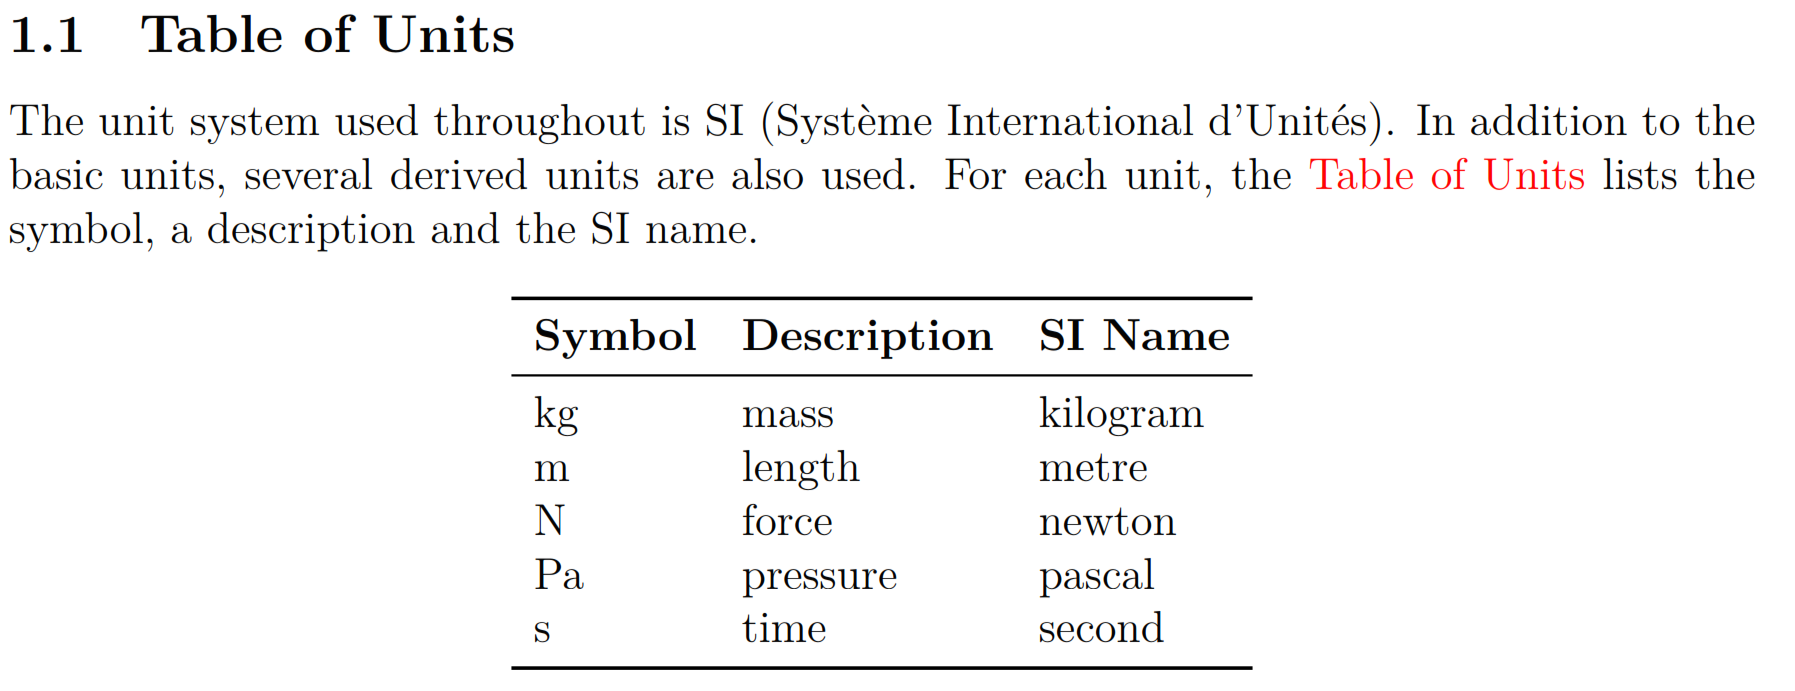
\includegraphics[width=\textwidth]{figures/gb_SRS_ToU.png}}
\caption{Table of Units Section}
\label{fig:gbrtou}
\end{subfigure}

\end{figure}

\begin{figure}\ContinuedFloat

\begin{subfigure}{\textwidth}
\centering
\fbox{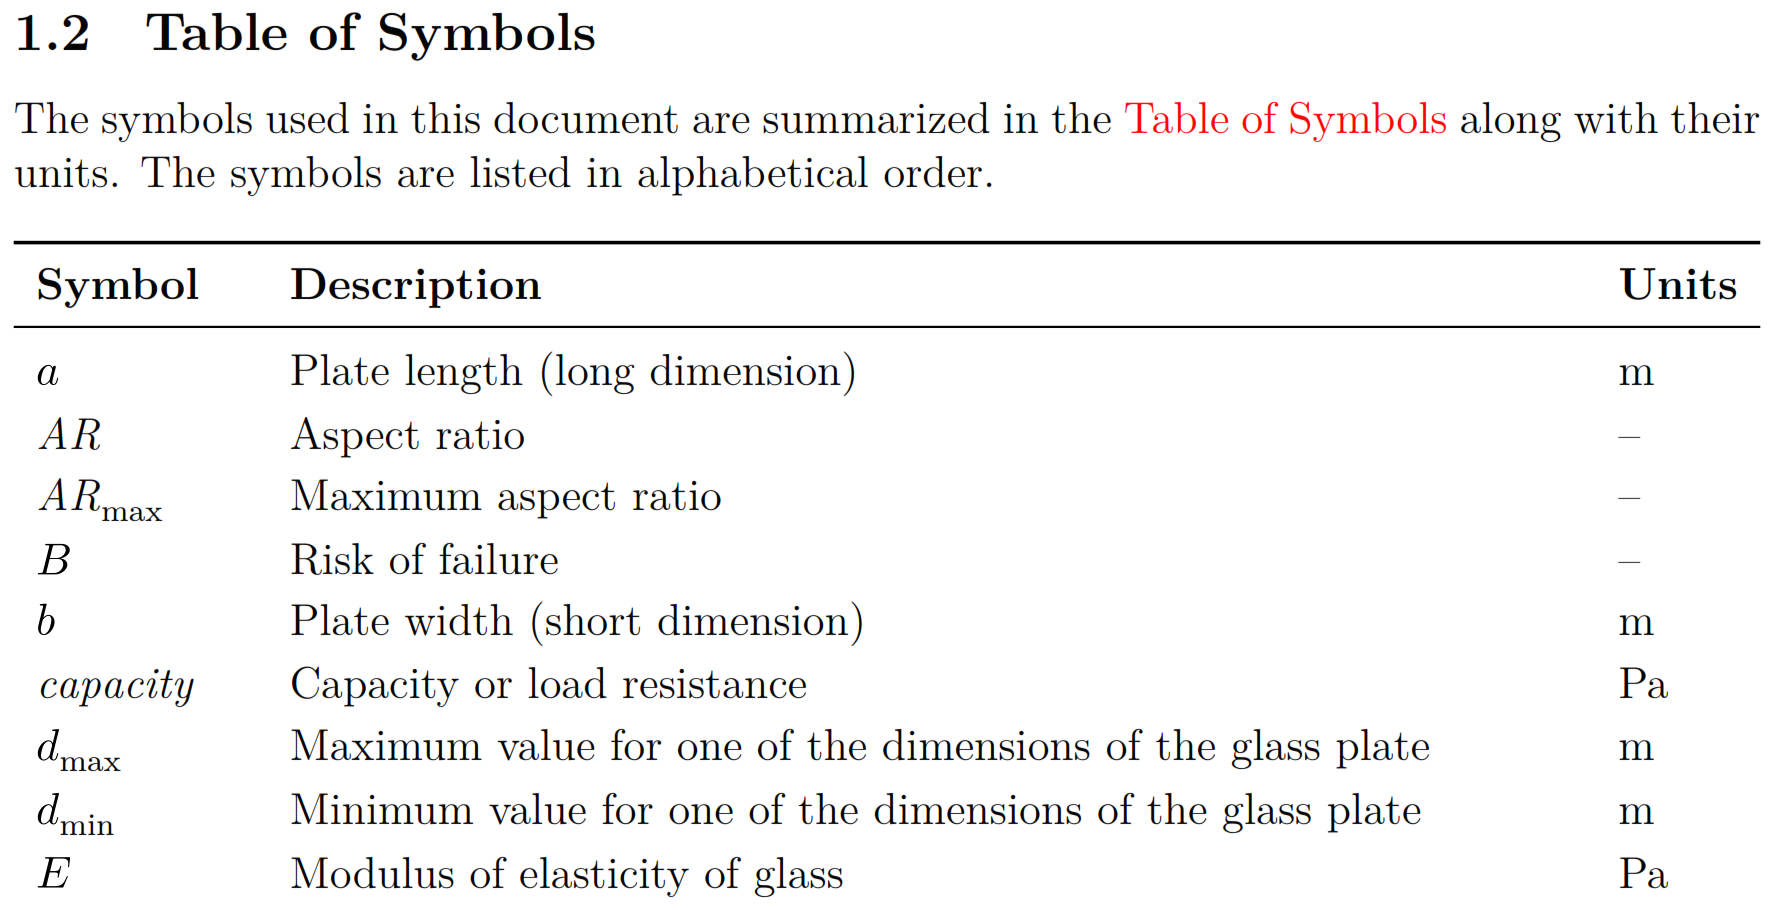
\includegraphics[width=\textwidth]{figures/gb_SRS_ToS.png}}
\caption{Table of Symbols (truncated) Section}
\label{fig:gbrtos}
\end{subfigure}


\begin{subfigure}{\textwidth}
\centering
\fbox{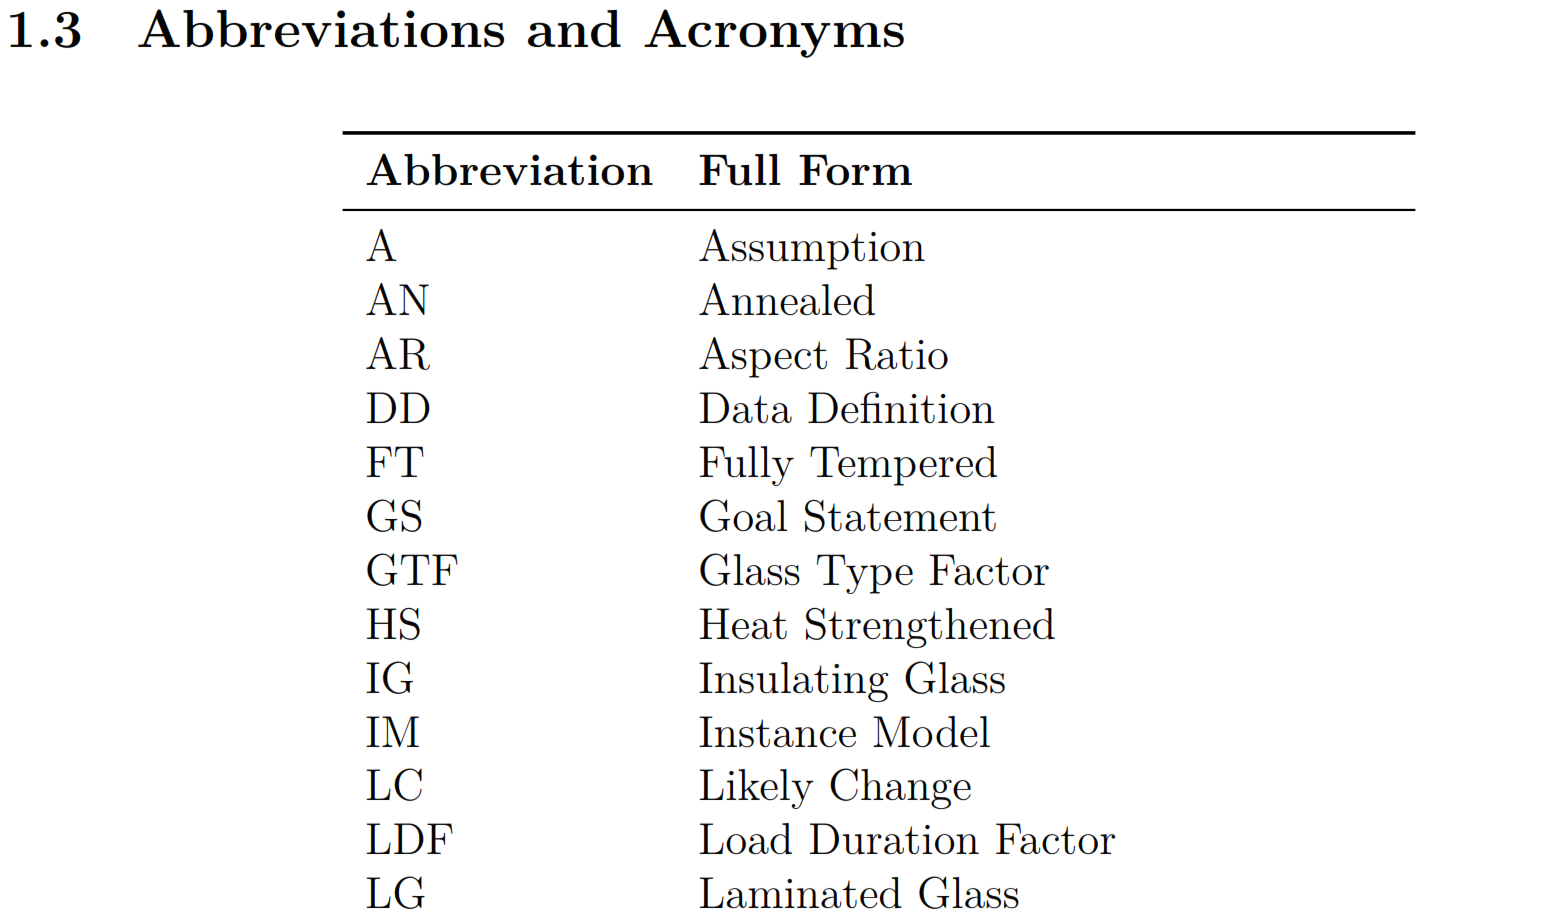
\includegraphics[width=\textwidth]{figures/gb_SRS_ToAA.png}}
\caption{Table of Abbreviations and Acronyms (truncated) Section}
\label{fig:gbrtoa}
\end{subfigure}
}
{The reference sections of \gb}
{fig:csRefSecs}

Looking at the (truncated for space) Table of Symbols, Table of Units, and 
Table of Abbreviations and Acronyms sections (Figure~\ref{fig:csRefSecs}) we 
can see that, barring the table values themselves, they are almost identical. 
The Table of Symbols is simply a table of values, akin to a glossary, specific 
to the symbols that appear throughout the rest of the document. For each of 
those symbols, we see the symbol itself, a brief description of what that 
symbol represents, and the units it is measured in, if applicable. Similarly, 
the Table of Units lists the Syst\`eme International d'Unit\'es (SI) Units used 
throughout the document, their descriptions, and the SI name. Finally, the 
table of Abbreviations and Acronyms lists the abbreviations and their full 
forms, which are essentially the symbols and their descriptions for each of the 
abbreviations.

While the reference material section should be fairly self-explanatory as to 
what it contains, other sections and subsections may not be so clear from their 
name alone. For example, it may not be clear offhand of what constitutes a 
theoretical model compared to a data definition or an instance model. One may 
argue that the author of the SRS, particularly if they chose to use the 
\smithea{} template, would need to understand that difference. However, it is 
not clear whether the intended audience would also have such an understanding. 
Who is that audience? Refer to Section~\ref{sec:sfs}, for more details. A brief 
summary is available in Table~\ref{tab:sfsummary}.

Returning to our exercise of breaking down each section of the SRS to determine 
the subtleties of \emph{what} is contained therein\footnote{The breakdown 
details are omitted for brevity and due to their monotonous nature, although 
the overall process is very much akin to the breakdown of the Reference 
Material section.} it should be unsurprising that each section maps to the 
definition provided in the \smithea{} template. However, as noted above, we can 
see distinct differences in the types of information contained in each section. 
Again we find some is boilerplate text meant to give a generic 
(non-system-specific) overview, some is specific to the proposed system, and 
some is in-between: it is specific to the problem domain for the proposed 
system, but not necessarily specific to the system itself.

Observing the contents of an SRS template adhere to said template may seem 
mundane, but it is a necessary step before we can move on to other \sfs{}. 
Without understanding what the SRS template intends to convey it is hard to 
assess weather or not the case study SRS conveys that information. With that in 
mind, we can move on to the MG and source code.

\ds{Current plan for following subsections: Brief description of the \sf{}, 
show an example of similarities within (ex. MG/MIS have a section per module, 
each section is organized the same way, some are filled in, some aren't), then 
follow a requirement through the MG to something in the MIS and finally to 
code. We'll dissect differences between case studies when looking at the 
patterns in Section~\ref{sec:patterns}. This also plants the seeds of "see, 
there's the same info moving from SRS $\rightarrow$ MG $\rightarrow$ MIS** 
$\rightarrow$ Code without stating it 
explicitly, which we can then do in the pattern section.}

\ds{Example to use should be a DD/IM from GlassBR, goes to calculations module 
in the MG, and finally a method in the source code}

\subsection{Module Guide}
\label{sec:breakdown:mg}

The module guide (MG) is a \sf{} that details the architecture of a given 
software system. It holds a number of design decisions around sensibly grouping 
functionalities within the system into modules to fulfill the requirements laid 
out in the SRS. For example, one might have an input/output module for handling 
user input and giving the user feedback through the display (ie. via print 
commands or some other output), or a calculations module that contains all of 
the calculation functions being performed in the normal operation of the given 
software system. The \smithea{} MG template also includes a traceability matrix 
for ease of verifying which requirements are fulfilled by which modules. 
Finally, the MG includes considerations for anticipated or unlikely changes 
that the system may undergo during its lifecycle.

\fig{
\begin{center}
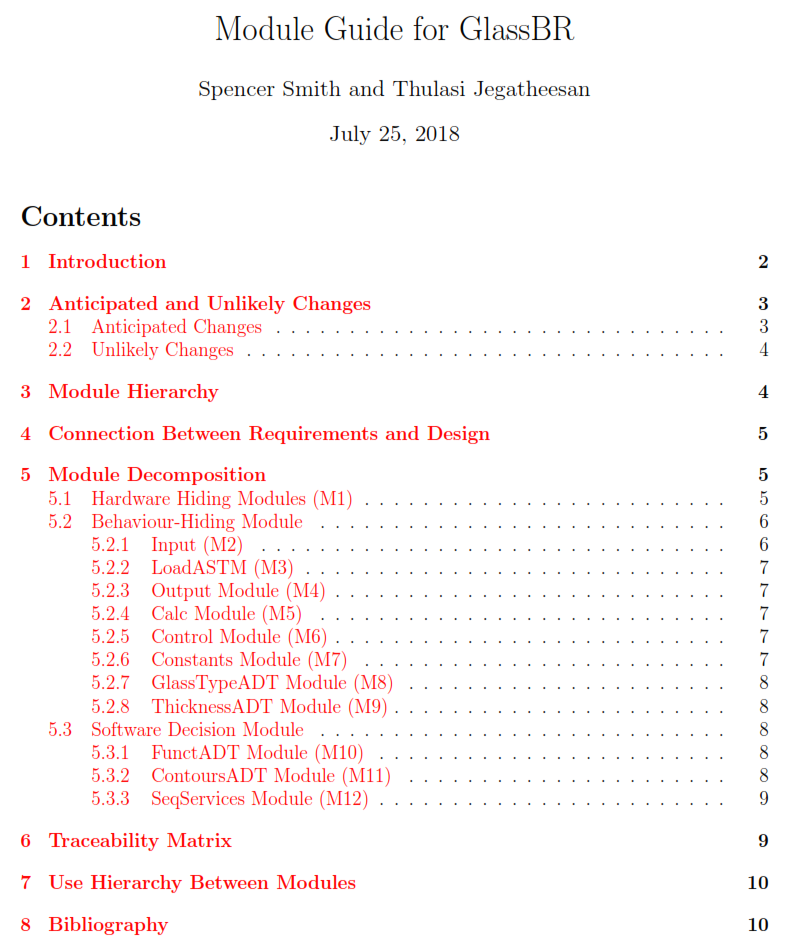
\includegraphics[width=\linewidth]{figures/gb_MG_ToC.png}
\end{center}}
{Table of Contents for GlassBR Module Guide}
{fig:gbrmgtoc}

Figure~\ref{fig:gbrmgtoc} shows the table of contents for the \gb{} case 
study's MG. For the sake of brevity we will omit the other case studies 
here (they can be found at \ds{TODO}). Just as with the SRS we are looking for 
commonality and understanding of what the document is trying to portray to the 
reader. As such we will ignore superficial differences between the MG sections. 
As the MG is a fairly short document we will look at each of the most relevant 
sections as part of this exercise.

Breaking down the MG by section, we can see that the introduction is itself 
completely generic boilerplate explaining the purpose of the MG, the audience, 
and some references to other works that explain why we would make certain 
choices over other (reasonable) ones given the opportunity. There is nothing 
system-specific, nor specific to the given problem domain of the case study.

Following through the table of contents into the ``Anticipated and Unlikely 
Changes" section, we see that again the introductions to this section and 
its subsections are generic boilerplate, however the details of each section 
are not. Both subsections are written in the same way: as a list of labeled 
changes (AC\# for anticipated change, UC\# for unlikely change). This is the 
first place we see both problem-domain and system-specific information 
Interestingly, the Module Hierarchy section follows the same general style: it 
is a list of modules which represent the leaves of the module hierarchy tree 
and each one is labeled (M\#).

\fig{
\begin{center}
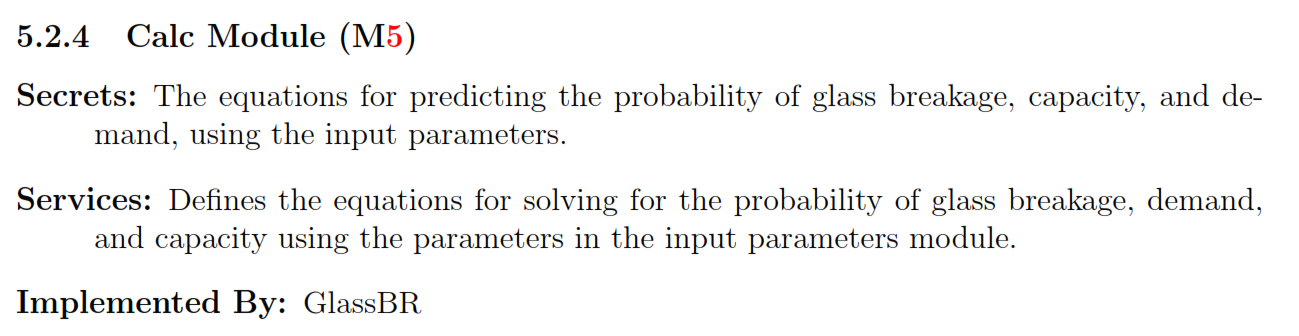
\includegraphics[width=\linewidth]{figures/gb_MG_CM.png}
\end{center}}
{Calc Module from the \gb{} Module Guide}
{fig:gbrmgcm}

Skipping ahead to the module decomposition, we find a section heading for each 
Level 1 module in the hierarchy, followed by subsections describing the Level 2 
modules. The former are almost entirely generic boilerplate (for example common 
Level 1 modules include: Hardware-Hiding, Behaviour-Hiding, and 
Software Decision modules), but the latter are problem-domain or system 
specific. An example of a system-specific module is shown in 
Figure~\ref{fig:gbrmgcm}. 

Each module is described by its secrets, services, and what it will be 
implemented by. For example, a given module could be implemented by the 
operating system (OS), the system being described (ex. \gb{}), or a third party 
system/library that will inter-operate with the given system.

Finally we have a traceability matrix and use hierarchy diagram. Both are 
visual representations of how the different modules implement the requirements 
and use each other respectively. The traceability matrix provides a direct and 
obvious link between the SRS and MG, where other connections between the two 
\sfs{} have been implicit until this point. Generally, the next \sf{} would be 
the MIS, however as it is structured so similarly to the MG (one section per 
module, each section organized in a very similar way, a repeated use hierarchy, 
etc) we will skip it for brevity. The MIS includes novel system-specific, 
implementation-level information denoting the interfaces between modules, but 
for our current exercise does not provide any revelations beyond that of the MG.

The MG gives us a very clear picture of \textit{decisions} made by the system 
designers, as opposed to the knowledge of the system domain, problem being 
solved, and requirements of an acceptable solution provided in the SRS. The MG 
provides platform and implementation-specific decisions, which will eventually 
be translated into implementation details in the source code. With that in 
mind, let us move on to the source code.

\subsection{Source Code}
\label{sec:breakdown:code}

The source code is arguably the most important \sf{} in any given software 
system since it serves as the set of instructions that a computer executes in 
order to solve the given problem. With only the other \sfs{} and without the 
source code, we would have a very well defined problem and acceptance criteria 
for a possible solution, but would never actually solve the problem.

\fig{
\begin{center}

\begin{forest}
  for tree={
    font=\ttfamily,
    grow'=0,
    child anchor=west,
    parent anchor=south,
    anchor=west,
    calign=first,
    edge path={
      \noexpand\path [draw, \forestoption{edge}]
      (!u.south west) +(7.5pt,0) |- node[fill,inner sep=1.25pt] {} (.child 
      anchor)\forestoption{edge label};
    },
    before typesetting nodes={
      if n=1
        {insert before={[,phantom]}}
        {}
    },
    fit=band,
    before computing xy={l=25pt},
  }
[/src/Python
  [Calc.py]
  [Constants.py]
  [ContoursADT.py]
  [Control.py]
  [Exceptions.py]
  [FunctADT.py]
  [GlassTypeADT.py]
  [Input.py]
  [LoadASTM.py]
  [Output.py]
  [SeqServices.py]
  [ThicknessADT.py]
]
\end{forest}

\end{center}
}
{Python source code directory structure for \gb{}}
{fig:gbsrcstruct}

As the source code is the executable set of instructions, one would expect it 
to be almost entirely system and problem-domain specific with very little 
boilerplate. Looking into the source of our case studies, we find this to be 
mostly true barring the most generic of library use (ex. 
\code{C}{stdio} in C).

Returning to our example of the MG from \gb{} (Figure~\ref{fig:gbrmgtoc}) and 
comparing it to the python source code structure shown in 
Figure~\ref{fig:gbsrcstruct} we can see that the source code follows almost 
identically in structure to the module decomposition. The only difference being 
the existence of an exceptions module defining the different types of
exceptions that may be thrown by the other modules. While this can be 
considered a fairly trivial difference, likely made for ease of maintenance, 
readability, and extensibility, it highlights that the two \sfs{} are out of 
sync. We speculate this difference was caused by a change made during the 
implementation phase, wherein the MG was not updated to reflect the addition of 
an exceptions module.

\fig{
\lstinputlisting[language=Python, firstline=5, 
lastline=61, firstnumber=5]{code/Calc.py}
}{Source code of the Calc.py module for \gb{}}{fig:gbrsrccalc}

Let us look deeper into the code for one specific module, for example the Calc 
module introduced in the MG~(Figure~\ref{fig:gbrmgcm}). The source code for 
said module can be found in Figure~\ref{fig:gbrsrccalc}. In the source code we 
see a number of calculation functions, including those that calculate the 
probability of glass breakage, demand (also known as \emph{load} or $q$), and 
capacity (also known as \emph{load resistance} or $LR$) as outlined in the 
\emph{secrets} section of the Calc module definition in the MG. We also see a 
number of intermediary calculation functions required to calculate these values 
(for example \code{python}|calc_NFL| and its dependencies).

The source code provides clear instructions to the machine on how to calculate 
each of these values and their intermediaries; it provides the actionable steps 
to solve the given problem. When we compare the code with relevant sections of 
the SRS, specifically the Data Definitions (DDs) for each term, we can see a 
very obvious transformation from one form to the other; the symbol used by the 
DD is the (partial) name of the function in the source code and the equation 
from the DD is calculated within the source code. This is one of many patterns 
we see across our \sfs{} within each case study.

\section{Identifying Repetitive Redundancy}
\label{sec:patterns}

From the examples in Section~\ref{sec:breakdown}, we can see a number of simple 
patterns emerging with respect to organization and information repetition 
within a case study. Upon applying our process to all of the case studies and 
adopting a broader perspective, numerous instances emerge where patterns 
transcend individual case studies and remain universally applicable. Several of 
these patterns should be unsurprising, as they relate to the template of a 
particular \sf{}. It is interesting, however, that patterns of information 
organization crop up within a given \sf{} in multiple places, containing 
distinct information.

Returning to our example from Section~\ref{sec:breakdown:srs}, looking only at 
the reference section of our SRS template, we have already found three 
subsections that contain the majority of their information in the same 
organizational structure: a table defining terms with respect to their symbolic 
representation and general information relevant to those terms. Additionally, 
we can see that the Table of Units and Table of Symbols have an introductory 
blurb preceding the tables themselves, whereas the Table of Abbreviations and 
Acronyms does not. Inspecting across case studies, we observe that the 
introduction to the Table of Units is nothing more than boilerplate text 
dropped into each case study verbatim; it is completely generic and applicable 
to \emph{any} software system using SI units. The introduction to the Table of 
Symbols also appears to be boilerplate across several examples, however, it 
does have minor variations which we can see by comparing 
Figure~\ref{fig:gbrtos} to Figure~\ref{fig:gptos} (\gb{} compared to \gp{}). 
These variations reveal the obvious: the variability between systems is greater 
than simply a difference in choice of symbols, and so there is some 
system-specific knowledge being encoded. While we can intuitively infer this 
conclusion based solely on each system addressing a different problem, our 
observation of the (structural) patterns within this SRS section confirms it.

\fig{
\centering
\fbox{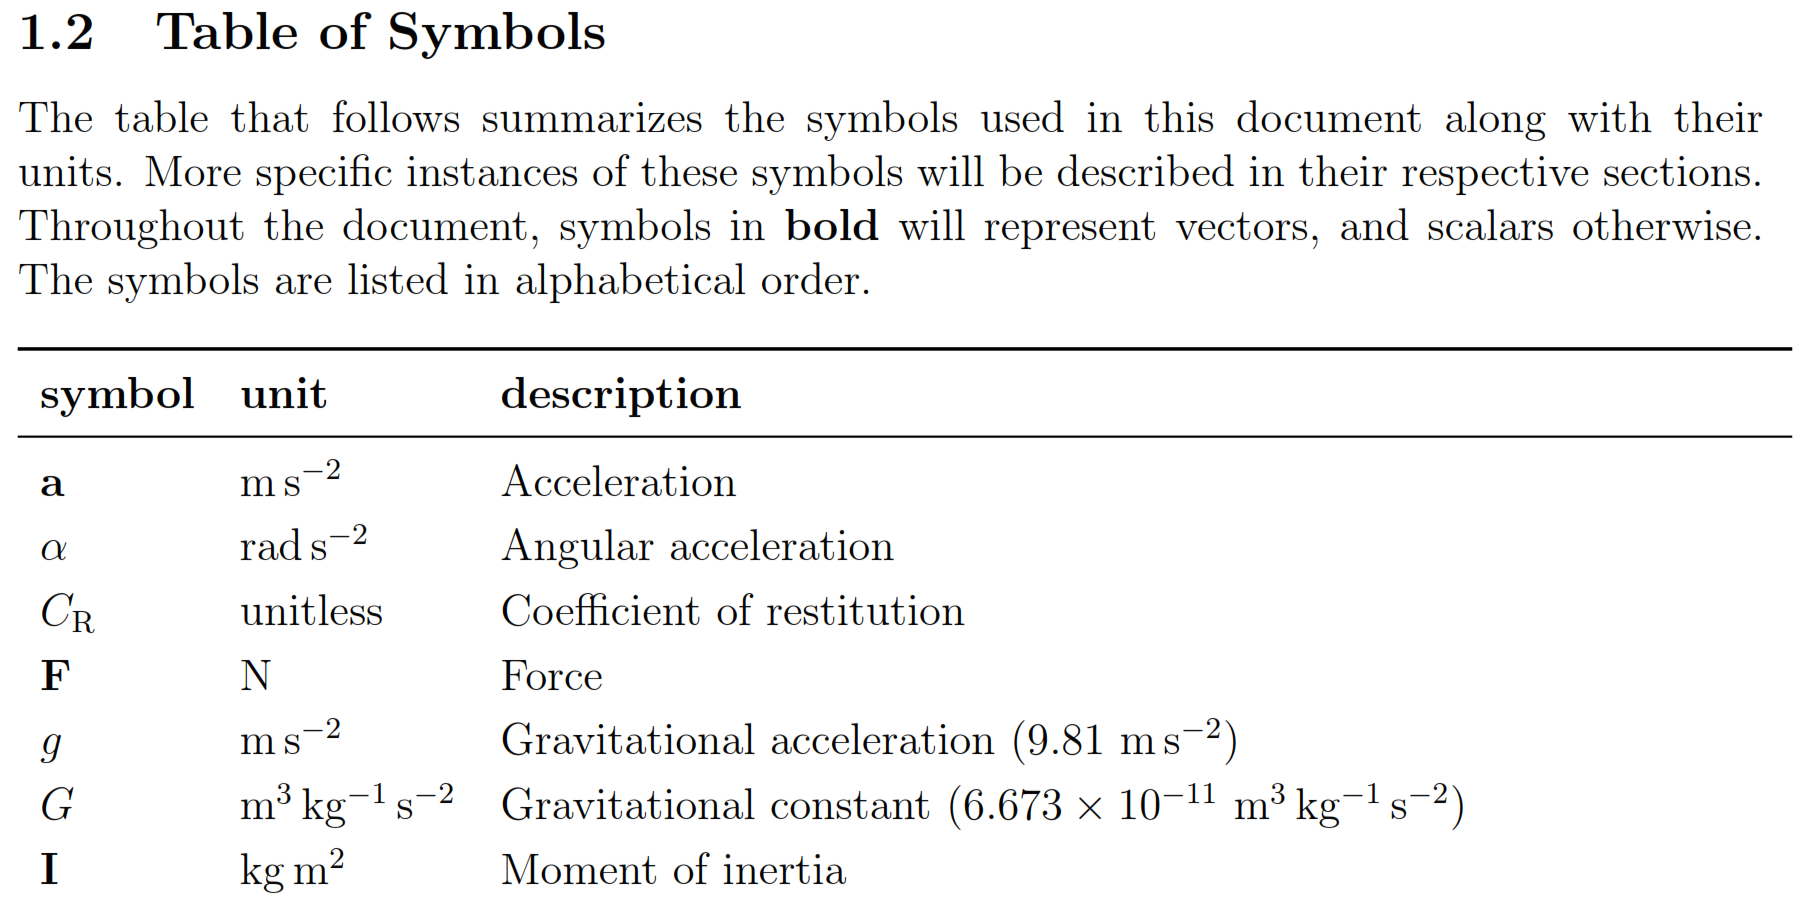
\includegraphics[width=\textwidth]{figures/gp_SRS_ToS.png}}
}
{Table of Symbols (truncated) Section from \gp{}}
{fig:gptos}

The reference section of the SRS provides a lot of knowledge in a very 
straightforward and organized manner. The basic units provided in the table of 
units give a prime example of fundamental, global knowledge shared across 
domains. Nearly any system involving physical quantities will use some of these 
units. On the other hand, the table of symbols provides system/problem-domain 
specific knowledge that will not be useful across unrelated domains. For 
example, the stress distribution factor $J$ from GlassBR may appear in several 
related problems, but would be unlikely to be seen in something like SWHS, 
NoPCM, or Projectile. Finally, acronyms are very context-dependent. They are 
often specific to a given domain and, without a coinciding definition, it can 
be very difficult for even the target audience to understand what they refer 
to. Within one domain, there may be several acronyms meaning different things, 
for example: PM can refer to a Product Manager, Project Manager, Program 
Manager, Portfolio Manager, etc.

By continuing to breakdown the SRS and other \sfs{}, we are able to find many 
more patterns. For example, we see the same concept being introduced in 
multiple areas within a single artifact and across artifacts in a project.
\fig{
\centering
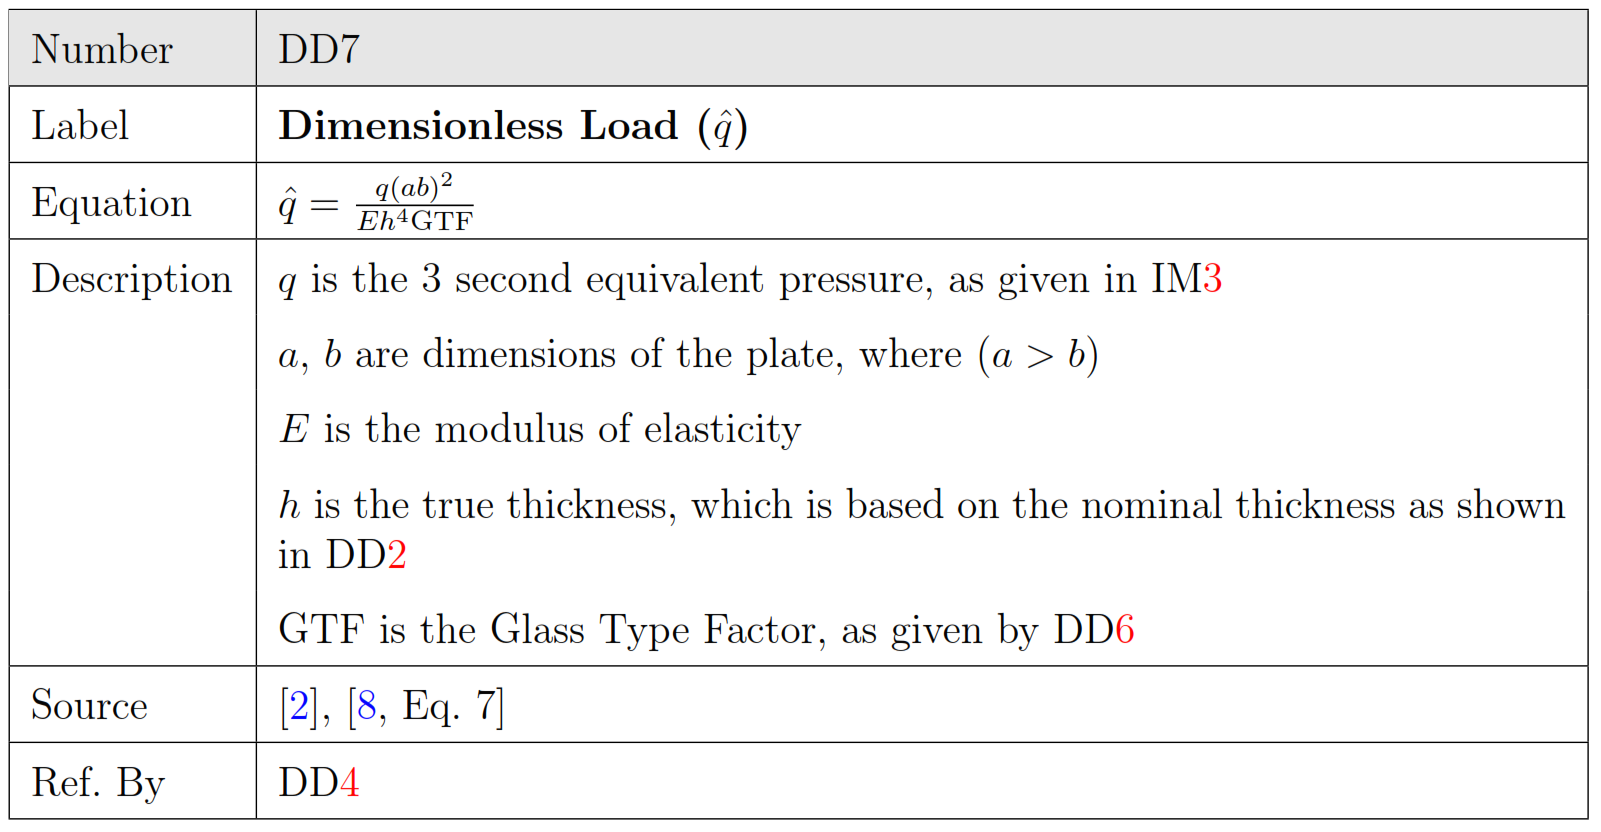
\includegraphics[width=\textwidth]{figures/gb_dd_q.png}}
{Data Definition for Dimensionless Load ($\hat{q}$) from \gb{} SRS}
{fig:gbrddq}
Figure~\ref{fig:gbrddq} shows the data definition for $\hat{q}$ in \gb{}. That 
same term was previously defined with fewer details in the table of symbols 
(omitted here for simplicity), as well as showing up implicitly or in passing 
in the MG (Figure~\ref{fig:gbrmgcm} and the \emph{loadASTM} module 
respectively), and implemented in the Source Code (Figure~\ref{fig:gbrsrccalc} 
lines 11-14). It should be noted that the SRS contains many references to 
$\hat{q}$, such as in the data definitions of the Stress Distribution Factor 
($J$) and Non-Factored Load ($NFL$). There are also implied references through 
intermediate calculations, for example the Calculation of Capacity ($LR$) is 
defined in terms of $NFL$ which relies on $\hat{q}$.

\ds{expand above to discuss knowledge projection/transformation and why things 
are the way they are above. word vomit:} %While $\hat{q}$ is only fully defined 
%for a human audience once, we need to keep some reference to it for different 
%audiences. It is expected each audience will understand the symbol in the 
%context of this system, or will be able to refer to the SRS to understand it 
%in more depth. For someone reading the SRS, the DD (and the reference 
%material) are important to quickly understand the full definition in the 
%context of the system's inputs, outputs, functional requirements, and 
%acceptance criteria. The MG barely mentions it, except in passing when 
%defining what the loadASTM and Calc modules are responsible for (the former 
%being loading values from a file, the latter using those values for 
%calculations). However the source code has a very detailed definition of it, 
%to ensure the computer is able to execute the appropriate calculation(s). The 
%varying level of detail throughout \sfs{} should not be too surprising as the 
%audience of each \sf{} requires a different level of verbosity depending on 
%their needs at any particular stage of the software development process. While 
%the verbosity varies, the underlying information is the same, ie. we are 
%always talking about $\hat{q}$ and what it represents regardless of the level 
%of detail we include. We are simply projecting relevant portions of our 
%knowledge of a given term based on our understanding of the context and our 
%audience's needs.
\ds{edited} 

Although the full definition of $\hat{q}$ is initially provided 
for a human audience only once, it is necessary to reference it in different 
ways for different audiences. Each audience is expected to grasp the symbol's 
meaning within their given context or consult other \sfs{} for more 
comprehensive understanding. When reading the SRS, the data definitions and 
other reference materials play a crucial role in swiftly comprehending the 
complete definition of $\hat{q}$ in relation to the system's inputs, outputs, 
functional requirements, and acceptance criteria.

The MG, on the other hand, briefly mentions $\hat{q}$ when defining the 
responsibilities of both the loadASTM and Calc modules (the former being 
responsible for loading values from a file, and the latter utilizing those 
values for calculations), whereas the source code provides a highly detailed 
definition to ensure accurate execution of the relevant calculation(s).

The varying level of detail across the \sfs{} should not come as a surprise 
since each \sf{} targets a different audience and their specific needs at 
various stages of the software development process. Although the level of 
verbosity may differ, the core information remains consistent: the authors are 
consistently referring to the definition of $\hat{q}$ via its representation, 
regardless of the level of detail incorporated. The goal is to convey relevant 
aspects of knowledge of a given term, while eliding that which is deemed 
superfluous, based on the context and the specific requirements of our 
audience. In other words, the authors only \emph{project} some portion of their 
knowledge of given terms at a given time, depending on their needs (precision, 
brevity, clarity, etc.), the expectations of the audience, and contextual 
relevance. \footnote{We have only referred to the term as $\hat{q}$ in this 
section to emphasize our argument and make the meta-point that the definition 
is irrelevant to our audience in this example. What matters is the symbolic 
reference, which we share a common understanding of.}

\ds{something about glossary = common example of a knowledge base w/ terms used 
for knowledge projections. That should go somewhere}

\ds{It all boils down to: Common Knowledge (system specific, domain specific, 
general/boilerplate) displayed via projections (decided on by artifact type and 
audience relevance) + organizational patterns}

If we broaden our view from a single system, to a software family, we can also 
find patterns of commonality across the various \sfs{} of the family members 
(For example the SWHS and NoPCM case studies) as they have been developed to 
solve similar, or in our case nearly identical, problems. Software family 
members are good examples to help determine what types of information or 
knowledge provided in the \sfs{} belong to the system-domain, problem-domain, 
or are simply general/boilerplate.

Looking at SWHS and NoPCM, we can easily find identical theoretical models 
(TMs) \ds{thermodynamics equations should look the same, use them here} as the 
underlying theory for each system is based on the problem domain.
However, when we follow the derivations from the TMs to the Instance Models 
(IMs), we find the resulting equations have changed due to the context of the 
system; the lack of PCM has changed the relevant equations for calculating the 
amount of heat energy stored in the tank as shown in 
Figure~\ref{fig:swhsnopcmim} \ds{Add figure 
showing the appropriate IM that has/lacks PCM in the equation}.

\ds{Patterns outlined above are a small subset of examples, but are highly 
generalizable}

While the above examples are fairly small and specific, they are indicative of 
a larger, more generalizable, set of patterns. Essentially, these patterns boil 
down to: Common knowledge (common to a system, domain, or \sfs{} as a whole) 
that has been transformed/projected through some means (incl. the identity 
projection) to provide relevant (to the audience and \sf{}) information; and 
patterns of organization within \sfs{}.

- inter-project (repetition throughout different views + other patterns.)
  vs intra-project knowledge (repetition across projects/family members,
  minor modifications, but fundamentally the same + other patterns.)
- Hint at chunkifying/parceling out the fundamental (system/view-agnostic)
knowledge vs the specific knowledge

\ds{\sout{Need to talk about knowledge projection/transformation in this section
- Use a relevant example from Case studies, maybe from PCM? Something like 
$\Delta{}U = Q - W$ is the same as ``Total energy within a closed system must 
be conserved" but transformed for / projects out what is relevant to a given 
audience.
- This will be useful for the following section} Covered that with the 
$\hat{q}$ example.}

\section{Organizing knowledge - a fluid approach}
  **Subsec roadmap:
    - We see the patterns above, we can generalize a lot of that
    - Direct repetition (copy-paste) vs indirect repetition (view-changes)
    require us to pull together knowledge from all artifacts into one place
    - Some can be derived automatically, the rest must be explicitly stated
    - We need to create a categorization system (hint at chunks) that is both
    robust and extensible to cover a wide variety of use cases.
    - Finally the templates give us structure

  **NOTE: Under the hood section should explain the process of how we determined
  what we needed to do. What we ended up doing should come in the following
  section(s) - no 'real' implementation details, only conceptual stuff here.

- Some ``boilerplate" information is actually in the domain of \sf{} writing 
and 
thus is so broad, yet relevant to everything we do, that we consider it 
completely general. Things like stakeholders, characteristics of the intended 
audience, etc.
  
\section{The seeds of Drasil}\ds{this'll probably get merged in to the previous 
section as a conclusion paragraph or something instead, unless I think of 
something big}
  **Subsec roadmap:
    -- Summarize the above subsections and lead into next section
    -- Add relevant information that doesn't quite fit above 
      and isn't implementation related
    -- 'Relevant buckshot section'

- We see patterns boil down to ``Give me relevant info on X for this \sf{} and 
audience" and ``Organize it in a reasonable way".

- Everything boils down to knowledge we are trying to convey, audience 
(context), and organizational structure. The latter can be 
handled through a number of means (deterministic generation / templates / 
blueprints). The former is more interesting as it essentially boils down to a 
particular grouping of information (knowledge-base) and some way to transform 
or project out what is relevant given a set of characteristics or expectations.